\newcommand*{\thead}[1]{\multicolumn{1}{|c|}{\bfseries #1}}

\chapter{Users}
An administrator (hereinafter referred to as admin) has to create/manage users in Obidos.
A user cannot assume the role of an admin.
Similarly an admin cannot assume the role of a user.
Users can store digital artifacts in Obidos.
Users must be explicitly granted permission by admin to manage Global Templates.

Users can be set up with single signon to corporate directory service (Active Directory or LDAP).
In such cases users can log into Obidos with their corporate username and password.
These users must have username registered in Obidos exactly as it appears in corporate Directory Service.
Since such accounts are meant to be single signon, the passwords are not set in Obidos; rather these
accounts are authenticated against the corporate Directory Service.

Users created with authentication done by Obidos are referred to as local accounts.
All admin accounts are local accounts. You can create local accounts for users.
Passwords for local accounts will follow the password policy in Obidos.

All types of active user accounts (local and maintained in corporate directory) are counted towards license limit.

\section{Create A User Account}

To create a user account, select "Create New User" item from the top "User Accounts" menu.

\begin{figure}[H]
\centering
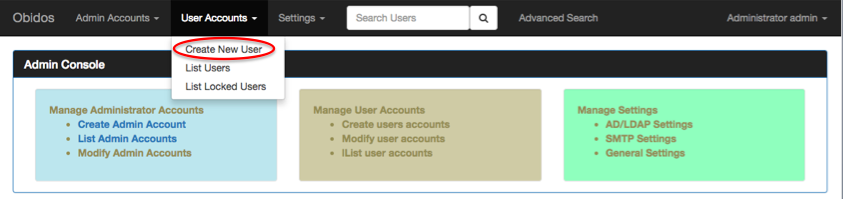
\includegraphics[width=90mm]{admin/New-User-Menu.png}
\caption{Create New User}
\label{fig: Figure}
\end{figure}

The admin has to fill in the details for the user.

\begin{figure}[H]
\centering
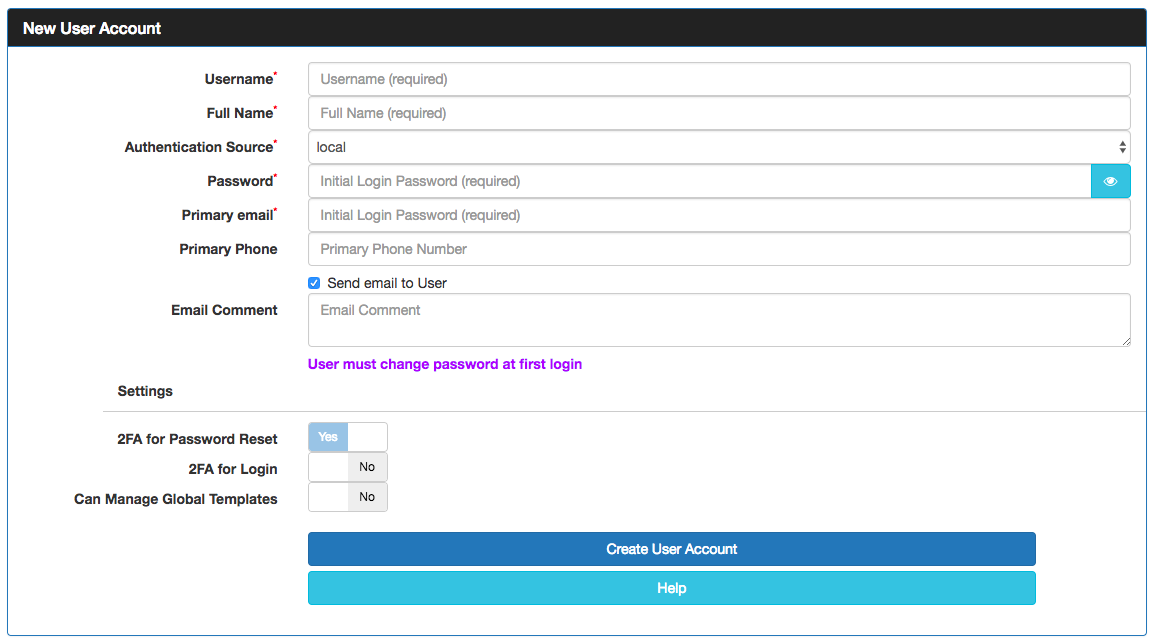
\includegraphics[width=90mm]{admin/Create-New-User.png}
\caption{New User Details}
\label{fig: Figure}
\end{figure}

\section{Bulk Importing Users (Only in Commerical Version)}

Large number of users can be imported to Obidos from command line as user \textbf{obidosadmin}. The user 
attributes must be defined in a file in LDIF format. The following attributes 
are required in the LDIF file:

\begin{center}
\begin{tabular}{|l|l|}
    \hline
    \thead{Attribute} & \thead{Maps to} \\
    \hline
    cn & Full name \\
    \hline
    mail & Email address \\
    \hline
    sAMAccountName & username \\
    \hline
    password & For local Obidos users only \\
    \hline
\end{tabular}
\end{center}

Before importing users, the following steps must be taken into account:

\begin{itemize}
    \item Make sure to dump the Obidos mariadb database in case something goes wrong.
    \item Make sure to configure SMTP setting in Obidos. By default, the initial 
password will be included in the notification email sent to the users.
    \item Make sure to configure AD/LDAP settings in Obidos if the users will be
imported from Active Directory or LDAP.
\end{itemize}

\subsection{Bulk Exporting and Importing Users from Active Directory}
The following are the steps to import users from Active Directory using ldif.

\begin{enumerate}
    \item Export users from AD using ldifde command on Windows.
    \item Upload the ldif file to Obidos server using the 'obidosadmin' account.
    \item Run the import\_users command to create accounts in Obidos.
\end{enumerate}

\subsubsection{Export Users from Active Directory}

Use the tool \href{https://docs.microsoft.com/en-us/previous-versions/windows/it-pro/windows-server-2012-  r2-and-2012/cc731033(v=ws.11}{ldifde}
to export users. Example:
\begin{verbatim}
    ldifde.exe -f adusers.ldif
\end{verbatim}

A sample LDIF file is shown below.

\begin{verbatim}
    dn: cn=Lloyd Kerluke
    cn: Lloyd Kerluke
    mail: lloyedka@example.com
    sAMAccountName: lloydk
    
    dn: cn=Marvin Cummerata
    cn: Marvin Cummerata
    mail: marvinc@example.com
    sAMAccountName: marvinc
    
    dn: cn=Annita Senger DC
    cn: Annita Senger DC
    mail: annitas@example.com
    sAMAccountName: annitas    
\end{verbatim}

\subsubsection{Upload the ldif file adusers.ldif to Obidos server}

Log in to the Obidos system using \textit{ssh} (or the web console) as the user \textbf{obidosadmin}. The
default password is \textbf{obidosadmin}. The password must be changed at the very first
login. It is a good idea to save the password in Obidos. 
Once the password has been changed for the obidosadmin user, use any sftp program
(or web console) to upload the adusers.ldif file to the Obidos server.

\subsubsection{Import users from adusers.ldif}

Be logged in to the Obidos server using \textit{ssh} or web console as \textbf{obidosadmin}. 
To see the usage of the import users program, run the following command:

\begin{verbatim}
$ import_users --help
usage: ImportUsers
    --ldapConfigName <ldapConfigName>   AD/LDAP Config name. Find it out
                                        from Settings > List AD/DLAP
                                        Settings. Requires for adding
                                        AD/LDAP users.
    --ldifFile <ldifFile>               LDIF file. Required.
    --noEmail                           Don't send initial password in
                                        notification email
    --requiers2FA                       2FA requires for password and
                                        passphrase reset
    --uidAttr <uidAttr>                 uid attribute. The default is
                                        sAMAccountName    
\end{verbatim}

\begin{itemize}
	\item To import AD/LDAP users into Obidos, type:
\end{itemize}

\begin{verbatim}
$ import_users \
    --ldapConfigName "AD Config Name" \
    --ldifFile adusers.ldif
\end{verbatim}
\textit{Note:} "AD Config Name" is the AD/LDAP configuration that you set up
as administrator in Obidos.
A notification email will be sent to the user. The users imported this way can log into
Obidos using their username and AD password.
\subsection{Creating multiple local Obidos users from ldif}
    If you just want to create multiple local Obidos users from an LDIF file:
\begin{enumerate}
    \item Create an ldif file with password field.
    \item Upload the file to Obidos server as the user obidosadmin.
    \item Run the import\_users command.
\end{enumerate}

\subsubsection{Create an LDIF file with the users.}
Use your favorite text editor to create the LDIF file. A sample LDIF file "localusers.ldif" with password is shown below. 

\begin{verbatim}
    dn: cn=Lloyd Kerluke
    cn: Lloyd Kerluke
    mail: lloyedka@example.com
    password: test
    sAMAccountName: lloydk
    
    dn: cn=Marvin Cummerata
    cn: Marvin Cummerata
    mail: marvinc@example.com
    password: test
    sAMAccountName: marvinc
    
    dn: cn=Annita Senger DC
    cn: Annita Senger DC
    mail: annitas@example.com
    password: test
    sAMAccountName: annitas    
\end{verbatim}

If the LDIF file does not have the \textbf{password} attribute, a random password
will be generated when the account is created in Obidos and will be included in the
notification email sent to the users. 
The users will be prompted to change the password at the first login to Obidos.

\subsubsection{Upload the ldif file to Obidos server.}
Using the obidosadmin account, upload the file "localusers.ldif" to the Obidos server.
\subsubsection{Import ldif users.}
Run the command 'import\_users' on the Obidos server after logging in (via ssh or web console) 
as the user 'obidosadmin'.
\begin{verbatim}
$ import_users \
    --ldifFile localusers.ldif
\end{verbatim}
The user will be prompted to change the password at the first login to Obidos application. 
\newpage
\section{List User Accounts}

In order to get the list of users, select "List Users" from top level "User Accounts" menu.
\begin{figure}[H]
\centering
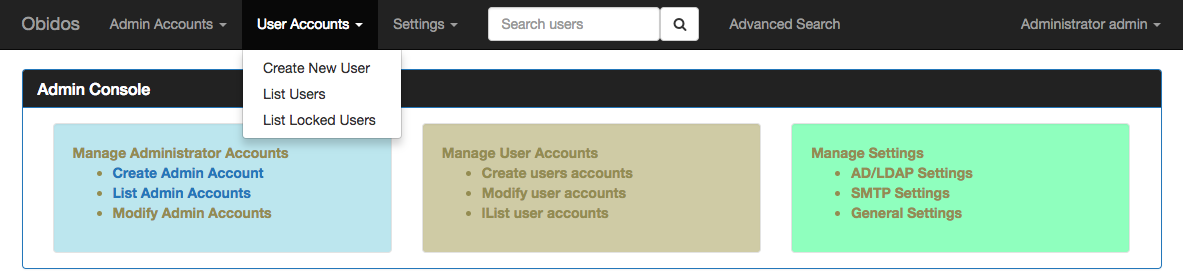
\includegraphics[width=90mm]{admin/User-Menu.png}
\caption{List User Menu}
\label{fig: Figure}
\end{figure}

The list of users will be displayed similar to the following figure.

\begin{figure}[H]
\centering
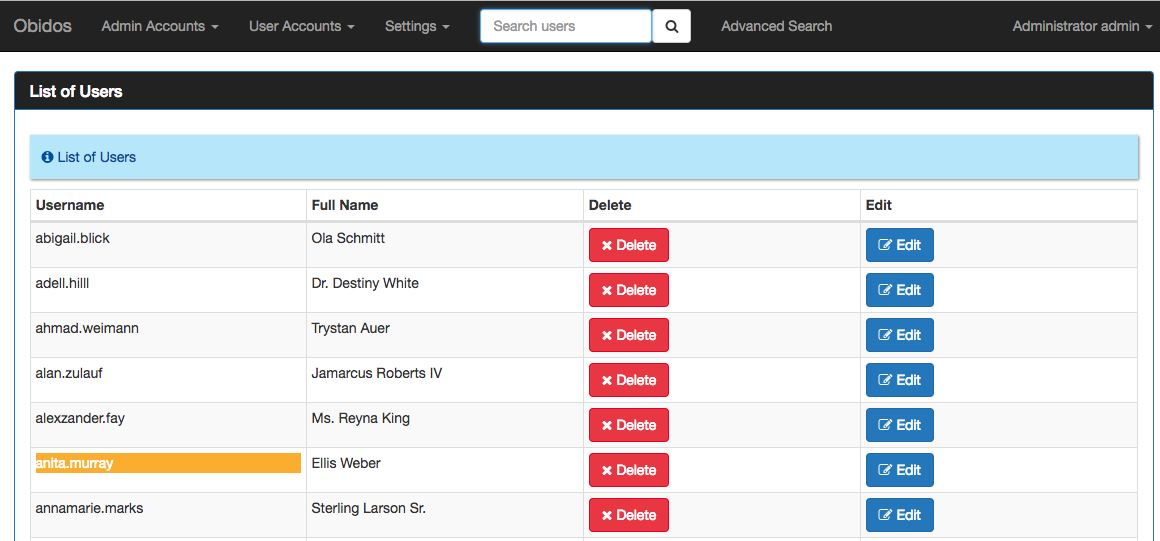
\includegraphics[width=90mm]{admin/List-Users.png}
\caption{List of Users}
\label{fig: Figure}
\end{figure}

\section{Reset User Password}

This action is allowed only for local accounts.
In the Edit User screen, there is option to reset password.

\begin{figure}[H]
\centering
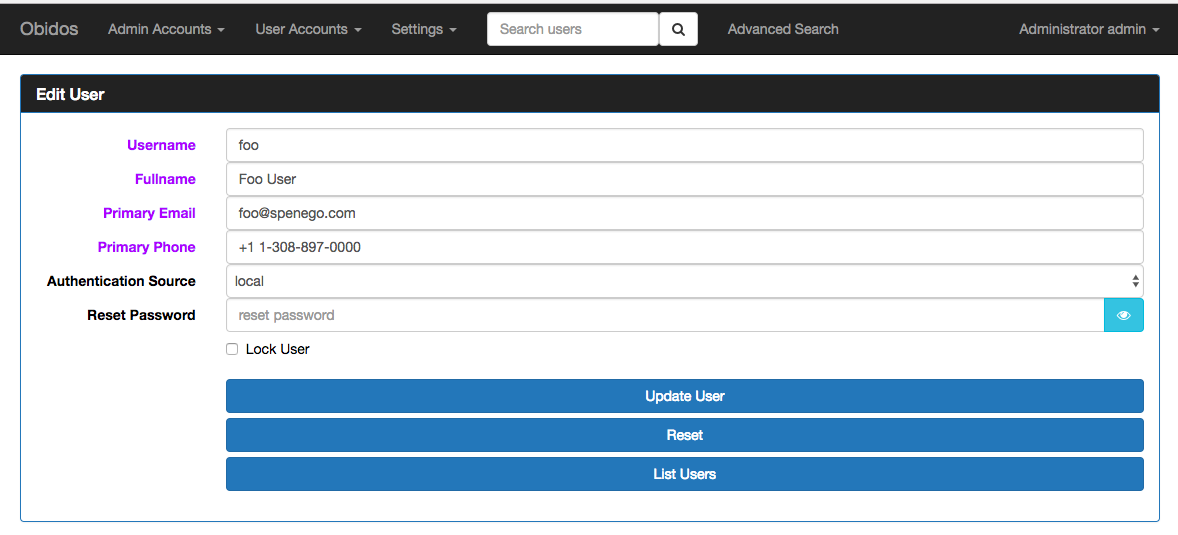
\includegraphics[width=90mm]{admin/Edit-User.png}
\caption{Reset Password}
\label{fig: Figure}
\end{figure}

\section{Lock a User Account}

This can be done from the screen for editing a user.
To do that, first select "List Users" from top level "User Accounts" menu.
From the list of users, click "Edit" button on the line corresponding to the user in the list.
When the edit menu shows up, there is a selection to Lock the user.
See the following figure.

\begin{figure}[H]
\centering
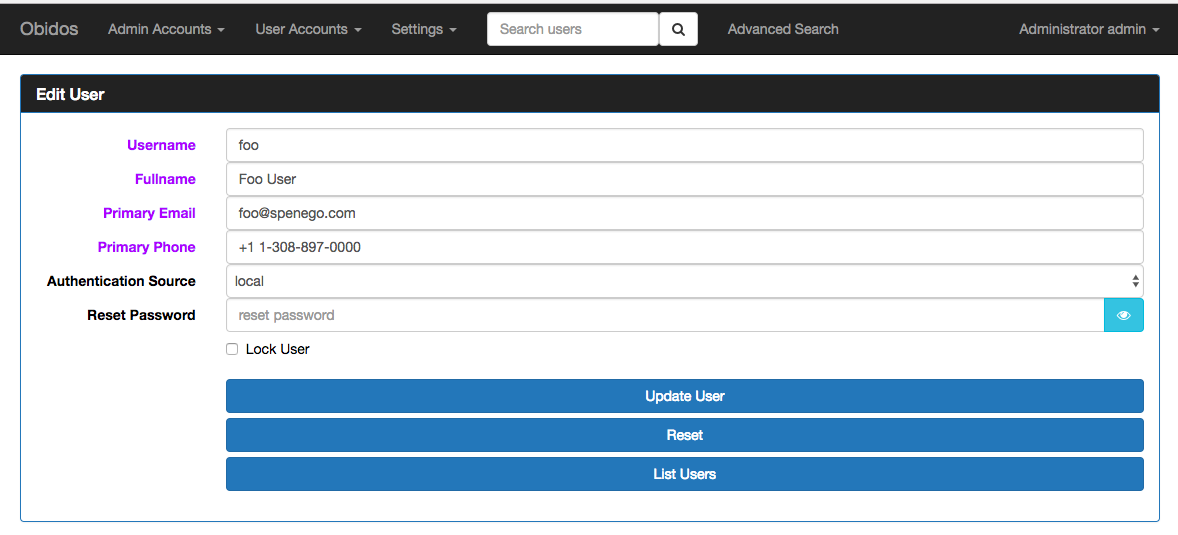
\includegraphics[width=90mm]{admin/Edit-User.png}
\caption{Lock User}
\label{fig: Figure}
\end{figure}

\section{Unlock a User Account}

Unlocking a User Account can be done only from the screen for editing a user account.
It is easy to the edit screen from the list of locked users.
The list of locked users can be obtained by selecting "List Locked Users" from top level "User Accounts" menu.
From the list of users, click "Edit" button on the line corresponding to the user in the list.
When the edit menu shows up, there is a selection to Unlock the user.
See the following figure.

\begin{figure}[H]
\centering
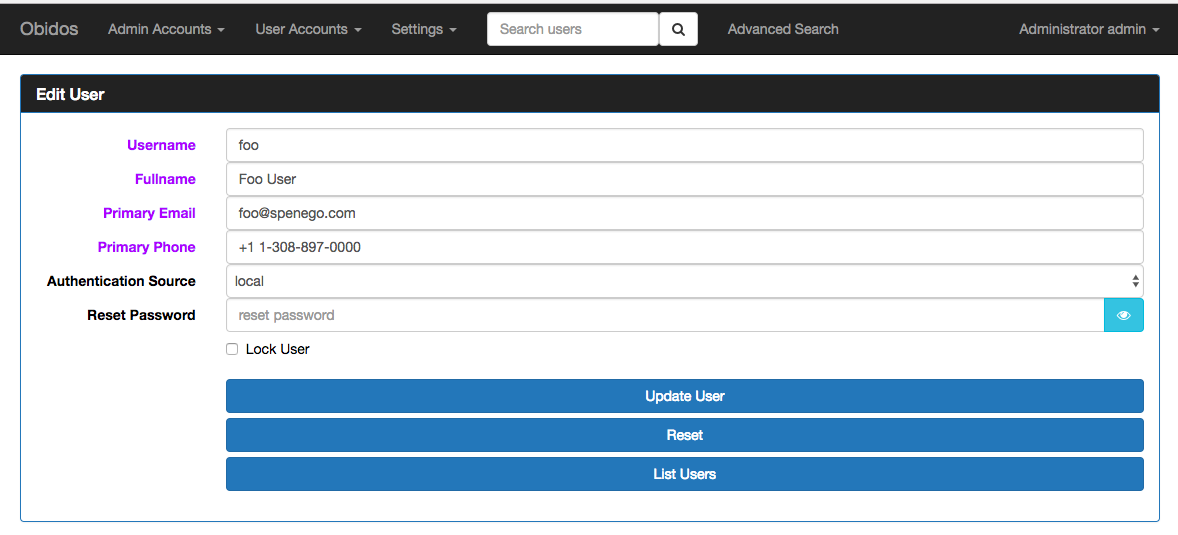
\includegraphics[width=90mm]{admin/Edit-User.png}
\caption{Unlock User}
\label{fig: Figure}
\end{figure}


\section{Tombstone a User Account}

Accounts can only be 'tombstoned'. They cannot be deleted.
To get to the "Tombstone" task, first the users must be listed.
This can be done by selecting "Manage Users" from the "Users" top navigation menu.
From the list of users, select the users of interest and click on "Tombstone" button.
A confirmation pop-up window will show up. Select "Yes" to confirm or "No" to cancel.
